\documentclass{article}
\usepackage[letterpaper,margin=0.5in]{geometry}
\usepackage{tikz}
\usepackage{amsmath,amssymb}
\usetikzlibrary{arrows.meta,positioning,shapes.geometric,fit,calc}

\begin{document}
\thispagestyle{empty}

\begin{figure*}[!t]
\centering
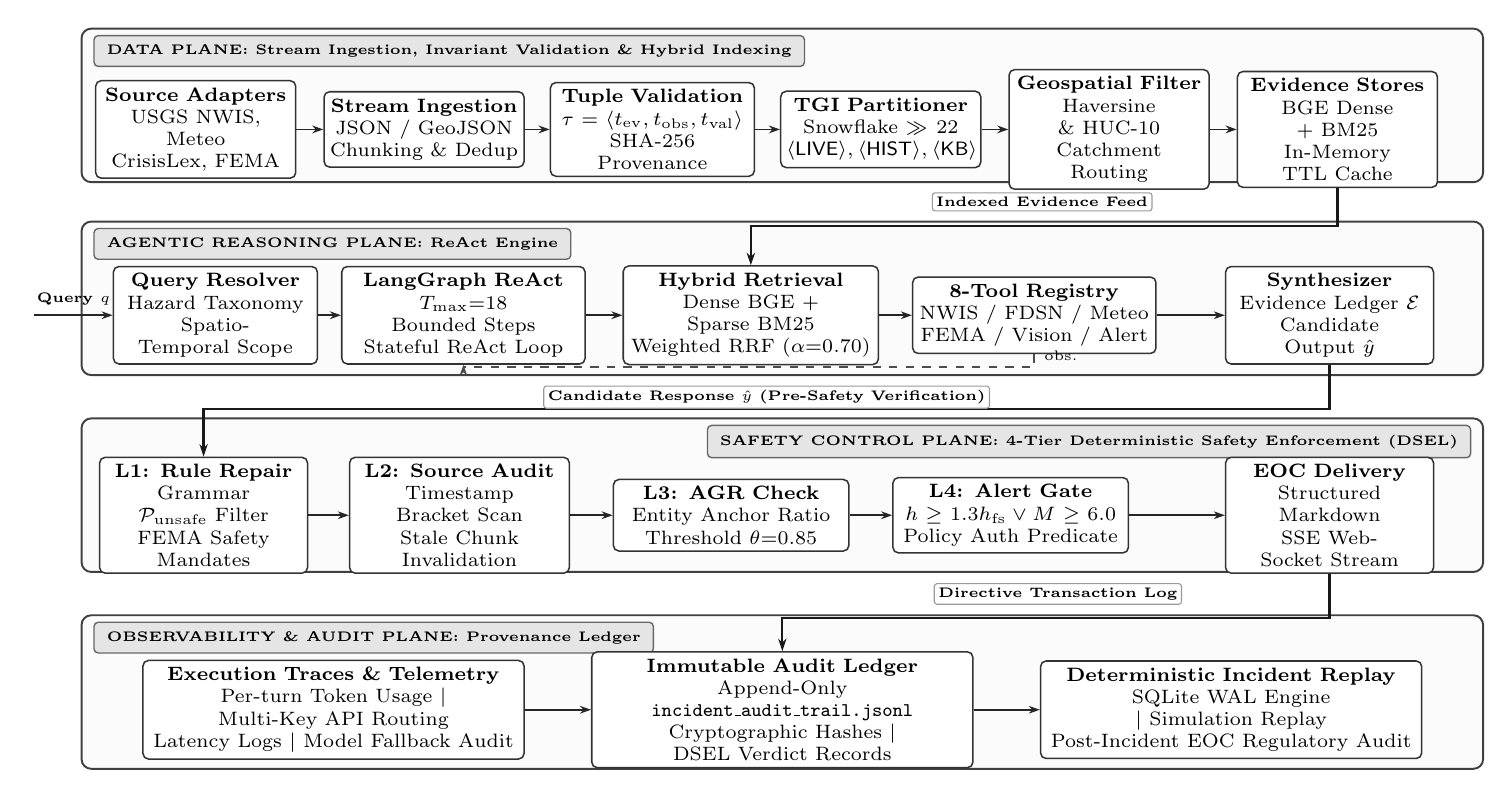
\begin{tikzpicture}[
  x=1cm, y=1cm, font=\scriptsize,
  plane/.style={draw=black!75, fill=gray!3, line width=0.7pt, rounded corners=3.5pt},
  tab/.style={draw=black!60, fill=gray!20, line width=0.5pt, rounded corners=1.5pt, font=\tiny\bfseries},
  comp/.style={draw=black!80, fill=white, line width=0.55pt, rounded corners=2pt,
               align=center, inner xsep=2pt, inner ysep=2.5pt, minimum height=0.88cm, font=\scriptsize},
  arr/.style={-{Stealth[length=4pt,width=2.8pt]}, line width=0.65pt, draw=black!85},
  dashedarr/.style={-{Stealth[length=4pt,width=2.8pt]}, line width=0.65pt, draw=black!70, dashed},
  interarr/.style={-{Stealth[length=4.5pt,width=3pt]}, line width=0.8pt, draw=black!90}
]

%% Total width: 17.80 cm.

%% =========================================================================
%% PLANE 1: DATA INGESTION & STORAGE PLANE  (y: 7.45 -> 9.40)
%% =========================================================================
\draw[plane] (0, 7.45) rectangle (17.80, 9.40);
\node[tab, anchor=north west] at (0.15, 9.32)
  {\,DATA PLANE: Stream Ingestion, Invariant Validation \& Hybrid Indexing\,};

\node[comp, text width=2.40cm] (src)   at ( 1.45, 8.12)
  {\textbf{Source Adapters}\\USGS NWIS, Meteo\\CrisisLex, FEMA};
\node[comp, text width=2.40cm] (ing)   at ( 4.35, 8.12)
  {\textbf{Stream Ingestion}\\JSON / GeoJSON\\Chunking \& Dedup};
\node[comp, text width=2.45cm] (qa)    at ( 7.25, 8.12)
  {\textbf{Tuple Validation}\\$\tau = \langle t_{\mathrm{ev}}, t_{\mathrm{obs}}, t_{\mathrm{val}} \rangle$\\SHA-256 Provenance};
\node[comp, text width=2.40cm] (tgi)   at (10.15, 8.12)
  {\textbf{TGI Partitioner}\\Snowflake $\gg 22$\\$\langle\mathsf{LIVE}\rangle, \langle\mathsf{HIST}\rangle, \langle\mathsf{KB}\rangle$};
\node[comp, text width=2.40cm] (geo)   at (13.05, 8.12)
  {\textbf{Geospatial Filter}\\Haversine \& HUC-10\\Catchment Routing};
\node[comp, text width=2.40cm] (store) at (15.95, 8.12)
  {\textbf{Evidence Stores}\\BGE Dense + BM25\\In-Memory TTL Cache};

\draw[arr] (src.east) -- (ing.west);
\draw[arr] (ing.east) -- (qa.west);
\draw[arr] (qa.east)  -- (tgi.west);
\draw[arr] (tgi.east) -- (geo.west);
\draw[arr] (geo.east) -- (store.west);

%% =========================================================================
%% PLANE 2: AGENTIC REASONING PLANE  (y: 5.00 -> 6.95)
%% =========================================================================
\draw[plane] (0, 5.00) rectangle (17.80, 6.95);
\node[tab, anchor=north west] at (0.15, 6.87)
  {\,AGENTIC REASONING PLANE: ReAct Engine\,};

\node[comp, text width=2.45cm] (qr)    at ( 1.70, 5.76)
  {\textbf{Query Resolver}\\Hazard Taxonomy\\Spatio-Temporal Scope};
\node[comp, text width=2.95cm] (react) at ( 4.85, 5.76)
  {\textbf{LangGraph ReAct}\\$T_{\max}{=}18$ Bounded Steps\\Stateful ReAct Loop};
\node[comp, text width=3.10cm] (retr)  at ( 8.50, 5.76)
  {\textbf{Hybrid Retrieval}\\Dense BGE + Sparse BM25\\Weighted RRF ($\alpha{=}0.70$)};
\node[comp, text width=2.95cm] (tools) at (12.10, 5.76)
  {\textbf{8-Tool Registry}\\NWIS / FDSN / Meteo\\FEMA / Vision / Alert};
\node[comp, text width=2.50cm] (synth) at (15.85, 5.76)
  {\textbf{Synthesizer}\\Evidence Ledger $\mathcal{E}$\\Candidate Output $\hat{y}$};

\draw[arr] (qr.east)    -- (react.west);
\draw[arr] (react.east) -- (retr.west);
\draw[arr] (retr.east)  -- (tools.west);
\draw[arr] (tools.east) -- (synth.west);

%% Clean external Query entrance from left:
\draw[arr] (-0.60, 5.76) -- node[above, font=\tiny\bfseries] {Query $q$} (qr.west);

%% Feed from Evidence Stores (Data Plane) into Hybrid Retrieval Engine:
\draw[interarr] (store.south) -- ++(0, -0.48) -| (retr.north);
\node[font=\tiny\bfseries, fill=white, inner sep=1.5pt, draw=black!40, rounded corners=1pt] at (12.20, 7.20) {Indexed Evidence Feed};

%% Tool Observation feedback loop back to ReAct (inside Plane 2)
\draw[dashedarr] (tools.south) -- ++(0, -0.16) node[pos=0.15, right, font=\tiny] {obs.} -| (react.south);

%% =========================================================================
%% PLANE 3: SAFETY CONTROL PLANE  (y: 2.50 -> 4.45)
%% =========================================================================
\draw[plane] (0, 2.50) rectangle (17.80, 4.45);
\node[tab, anchor=north east] at (17.65, 4.37)
  {\,SAFETY CONTROL PLANE: 4-Tier Deterministic Safety Enforcement (DSEL)\,};

\node[comp, text width=2.50cm] (l1) at ( 1.55, 3.22)
  {\textbf{L1: Rule Repair}\\Grammar $\mathcal{P}_{\text{unsafe}}$ Filter\\FEMA Safety Mandates};
\node[comp, text width=2.65cm] (l2) at ( 4.80, 3.22)
  {\textbf{L2: Source Audit}\\Timestamp Bracket Scan\\Stale Chunk Invalidation};
\node[comp, text width=2.85cm] (l3) at ( 8.25, 3.22)
  {\textbf{L3: AGR Check}\\Entity Anchor Ratio\\Threshold $\theta{=}0.85$};
\node[comp, text width=2.85cm] (l4) at (11.80, 3.22)
  {\textbf{L4: Alert Gate}\\$h \ge 1.3h_{\text{fs}} \lor M \ge 6.0$\\Policy Auth Predicate};
\node[comp, text width=2.50cm] (eoc) at (15.85, 3.22)
  {\textbf{EOC Delivery}\\Structured Markdown\\SSE WebSocket Stream};

\draw[arr] (l1.east) -- (l2.west);
\draw[arr] (l2.east) -- (l3.west);
\draw[arr] (l3.east) -- (l4.west);
\draw[arr] (l4.east) -- (eoc.west);

%% Candidate response from Synthesizer into Safety Plane (L1):
\draw[interarr] (synth.south) -- ++(0, -0.56) -| (l1.north);
\node[font=\tiny\bfseries, fill=white, inner sep=1.5pt, draw=black!40, rounded corners=1pt] at (8.70, 4.72) {Candidate Response $\hat{y}$ (Pre-Safety Verification)};

%% =========================================================================
%% PLANE 4: OBSERVABILITY & AUDIT PLANE  (y: 0.00 -> 1.95)
%% =========================================================================
\draw[plane] (0, 0.00) rectangle (17.80, 1.95);
\node[tab, anchor=north west] at (0.15, 1.87)
  {\,OBSERVABILITY \& AUDIT PLANE: Provenance Ledger\,};

\node[comp, text width=4.70cm] (trace) at ( 3.20, 0.75)
  {\textbf{Execution Traces \& Telemetry}\\Per-turn Token Usage \textbar\ Multi-Key API Routing\\Latency Logs \textbar\ Model Fallback Audit};
\node[comp, text width=4.70cm] (alog)  at ( 8.90, 0.75)
  {\textbf{Immutable Audit Ledger}\\Append-Only \texttt{incident\_audit\_trail.jsonl}\\Cryptographic Hashes \textbar\ DSEL Verdict Records};
\node[comp, text width=4.70cm] (replay) at (14.60, 0.75)
  {\textbf{Deterministic Incident Replay}\\SQLite WAL Engine \textbar\ Simulation Replay\\Post-Incident EOC Regulatory Audit};

\draw[arr] (trace.east)  -- (alog.west);
\draw[arr] (alog.east)   -- (replay.west);

%% Clean logging connection: EOC delivery logs transactions into Audit Ledger:
\draw[interarr] (eoc.south) -- ++(0, -0.56) -| (alog.north);
\node[font=\tiny\bfseries, fill=white, inner sep=1.5pt, draw=black!40, rounded corners=1pt] at (12.40, 2.22) {Directive Transaction Log};

\end{tikzpicture}
\end{figure*}
\end{document}
